\documentclass[a4paper]{article}

\usepackage[english]{babel}
\usepackage[utf8x]{inputenc}
\usepackage{graphicx}
\usepackage{xcolor}
\usepackage[colorinlistoftodos]{todonotes}
\usepackage{float}
\usepackage[normalem]{ulem}
\usepackage{hyperref}
\hypersetup{colorlinks,urlcolor=blue}

% hack into hyperref
\makeatletter
\DeclareUrlCommand\ULurl@@{%
  \def\UrlFont{\ttfamily\color{blue}}%
  \def\UrlLeft{\uline\bgroup}%
  \def\UrlRight{\egroup}}
\def\ULurl@#1{\hyper@linkurl{\ULurl@@{#1}}{#1}}
\DeclareRobustCommand*\ULurl{\hyper@normalise\ULurl@}
\makeatother

\title{Astro Note}
\author{Marek Bielik}

\begin{document}
\maketitle

\section*{Basic description}
Astro Note is a very simple tool, that let's users make notes of their night-sky observations. If you're an astronomer, you are certainly familiar with \href{https://en.wikipedia.org/wiki/List_of_Messier_objects}{Messier catalog}. This app uses a remote database to retrieve a list of currently visible Messier objects and shows information about certain objects. Then you can add the object in your collection and make your note about the observation. Objects which you already have within your trophies will be ticked, or alternatively, you can display all your trophies and edit the notes if you wish. \newline \newline
App will use the internet in order to connect to the remote database and to display images of Messier objects. User interface will be based on Fragments in cooperation with Activities, so that user will be able to swipe between screens. \newline \newline

\section*{Database description}
The database used in the app will consist of one table:
\begin{verbatim}
CREATE TABLE MessierObjects (
  MessierNumber INTEGER PRIMARY KEY,
  NGC TEXT,
  CommonName TEXT,
  PictureURL TEXT,
  Type TEXT,
  Constellation TEXT,
  ApparentMagnitude REAL,
  Note TEXT
);
\end{verbatim}
Every Messier object has it's unique number in the list, so there's no need to generate them. All the attributes will be copied from the remote database, except the Note attribute, this will be set / updated by user. Application will show a picture of every Messier object, these pictures will be loaded from the internet, so there are only URL's in the database.

\section*{Use Case diagram}
\begin{figure}[H]
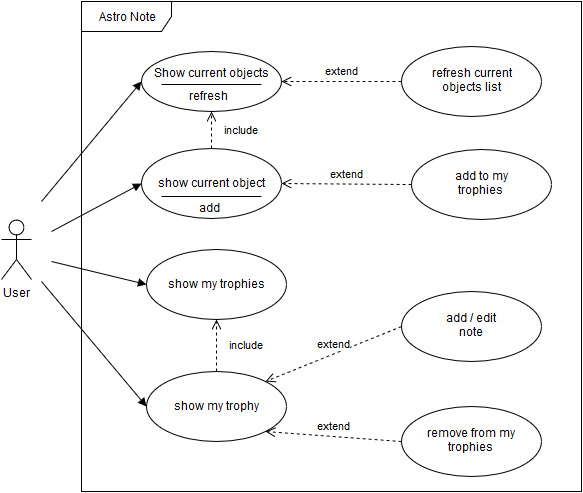
\includegraphics[width=\textwidth]{AstroNoteUseCase.png}
\end{figure}

\section*{Basic screen flow}
\begin{figure}[H]
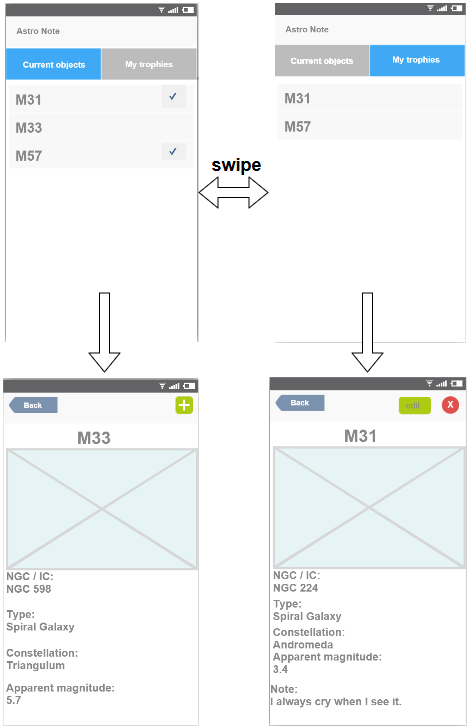
\includegraphics[width=\textwidth]{AstroNoteScreens.png}
\end{figure}
\end{document}